\documentclass[avery5371, grid,frame]{flashcards}

\usepackage{graphicx}
\usepackage{geometry}

\geometry{a4paper, landscape, margin=0.2in}
\cardfrontstyle[\large\slshape]{headings}
\cardbackstyle{empty}

\begin{document}

\renewcommand{\cardpaper}{a4paper}
\renewcommand{\cardpapermode}{landscape}
\renewcommand{\cardrows}{2}
\renewcommand{\cardcolumns}{2}
\setlength{\cardheight}{3.5in}
\setlength{\cardwidth}{5.0in}
\setlength{\topoffset}{0.50in}
\setlength{\oddoffset}{0.50in}
\setlength{\evenoffset}{0.50in}

\begin{flashcard}{medicine}
    \vspace*{\fill}
    \begin{center}
        \begin{minipage}[c]{.45\textwidth}
            
\includegraphics[width=\textwidth]{cards/m/medicine/medicine - a doctor holding a giant pill, ready to administer it.png}
        \end{minipage}
        \begin{minipage}[c]{.45\textwidth}
            \begin{itemize}\setlength\itemsep{12pt}
            \item Explanation: \ A substance used to treat a disease or condition.

            \item Example: \ a doctor holding a giant pill, ready to administer it
            \end{itemize}
        \end{minipage}
    \end{center}
    \vspace*{\fill}
\end{flashcard}\begin{flashcard}{medicine}
    \vspace*{\fill}
    \begin{center}
        \begin{minipage}[c]{.45\textwidth}
            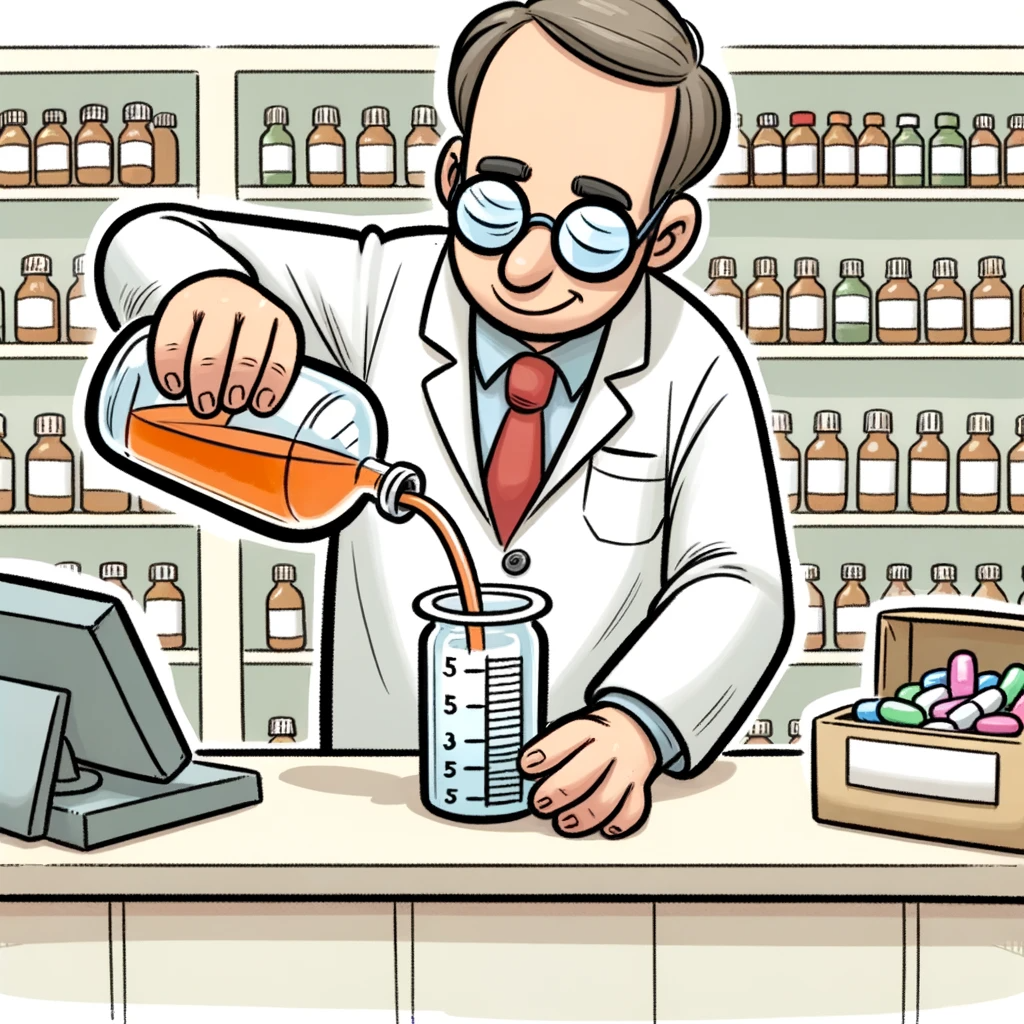
\includegraphics[width=\textwidth]{cards/m/medicine/medicine - a pharmacist behind a counter, measuring out liquid medicine into a bottle.png}
        \end{minipage}
        \begin{minipage}[c]{.45\textwidth}
            \begin{itemize}\setlength\itemsep{12pt}
            \item Explanation: \ A substance used to treat a disease or condition.

            \item Example: \ a pharmacist behind a counter, measuring out liquid medicine into a bottle
            \end{itemize}
        \end{minipage}
    \end{center}
    \vspace*{\fill}
\end{flashcard}\begin{flashcard}{medicine}
    \vspace*{\fill}
    \begin{center}
        \begin{minipage}[c]{.45\textwidth}
            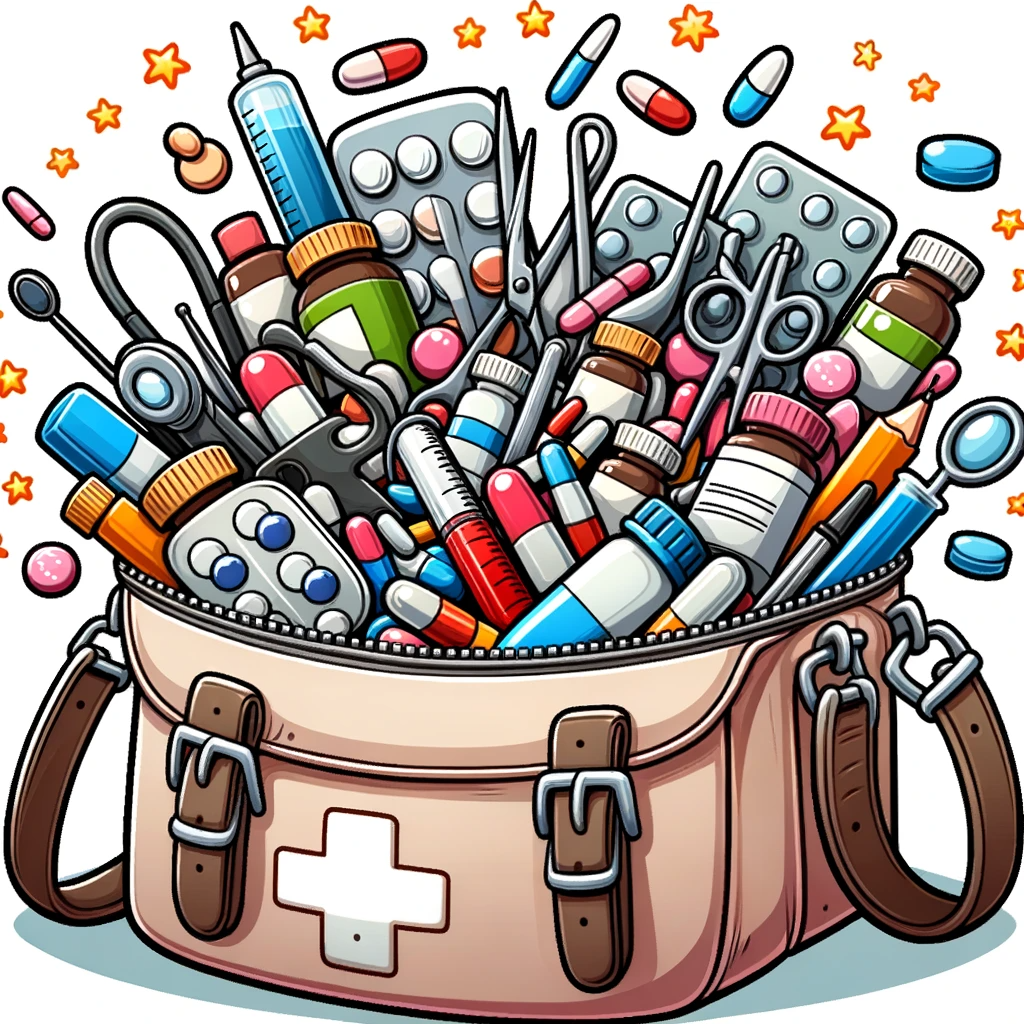
\includegraphics[width=\textwidth]{cards/m/medicine/medicine - a medical bag overflowing with various medical tools and bottles of pills.png}
        \end{minipage}
        \begin{minipage}[c]{.45\textwidth}
            \begin{itemize}\setlength\itemsep{12pt}
            \item Explanation: \ A substance used to treat a disease or condition.

            \item Example: \ a medical bag overflowing with various medical tools and bottles of pills
            \end{itemize}
        \end{minipage}
    \end{center}
    \vspace*{\fill}
\end{flashcard}\begin{flashcard}{medicine}
    \vspace*{\fill}
    \begin{center}
        \begin{minipage}[c]{.45\textwidth}
            
\includegraphics[width=\textwidth]{cards/m/medicine/medicine - a child looking at a spoonful of syrupy medicine with a curious expression.png}
        \end{minipage}
        \begin{minipage}[c]{.45\textwidth}
            \begin{itemize}\setlength\itemsep{12pt}
            \item Explanation: \ A substance used to treat a disease or condition.

            \item Example: \ a child looking at a spoonful of syrupy medicine with a curious expression
            \end{itemize}
        \end{minipage}
    \end{center}
    \vspace*{\fill}
\end{flashcard}

\end{document}